\item A car is traveling on a straight road, with a velocity given by the graph below.  Here, velocity is measured in miles per hour and time is measured in hours.  Positive velocity means movement to the right, negative velocity means movement to the left.

What is the displacement of the car in miles during the time period $0 \leq t \leq 5$ ?



\begin{center}
	
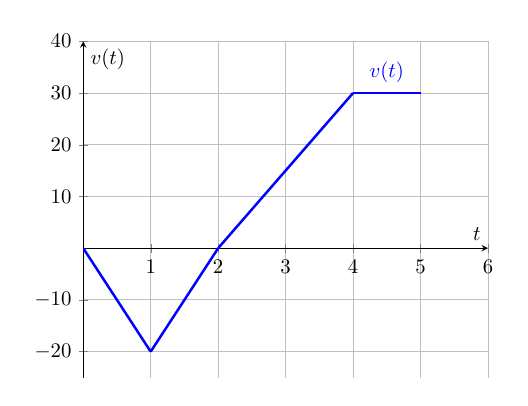
\begin{tikzpicture}[scale=0.75]
\begin{axis}[grid=both,
	axis x line=middle,
	axis y line=center,
	xmin=0,
	xmax=6,
	ymin=-25,
	ymax=40,
	xlabel=$t$,ylabel=$v(t)$,
	xtick={0,1,2,3,4,5,6},
	ytick={-20,-10,10,20,30,40}
]
\addplot[very thick,blue,mark=none,
	 domain=0:1,samples=100]
	{-1*20*x};
\addplot[very thick,blue,mark=none,
	 domain=1:2,samples=100]
	{20*(x-2)};
\addplot[very thick,blue,mark=none,
	 domain=2:4,samples=100]
	{15*(x-2)};

	\addplot[very thick,blue,mark=none,
	 domain=4:5,samples=100]
	{30};


	\node[blue] at (axis cs:4.5,34){$v(t)$};
\end{axis}
\end{tikzpicture}
\end{center}

\begin{multicols}{2}
	\begin{enumerate}
	\item $40$ miles % correct
	\item $60$ miles
	\item $80$ miles
	\item There is not enough information to find the displacement.
	% \item None of the above.
	\end{enumerate}
\end{multicols}
